%%%%%%%%%%%%%%%%%%%%%%%%%%%%%%%%%%%%%%%%%%%%%%%%%
%
% Universita' degli Studi dell'Insubria
%
%%%%%%%%%%%%%%%%%%%%%%%%%%%%%%%%%%%%%%%%%%%%%%%%%

\documentclass[a4paper, 11pt, oneside]{book}
\usepackage[a4paper]{geometry}
\usepackage{lmodern}
\usepackage[italian]{babel}
\usepackage{textcomp}
\usepackage{color}
\usepackage{url}
\usepackage{amsfonts}
\usepackage{float}
\usepackage{booktabs}
\usepackage{longtable}
\usepackage{makeidx}
\usepackage{fancyhdr}
\usepackage[times]{quotchap}
\usepackage{multirow}
\usepackage{version}

\usepackage{listings}
\lstdefinestyle{DOS}{
	backgroundcolor=\color{lightgray!15},
	basicstyle=\scriptsize\ttfamily
}
\usepackage{color}
\usepackage{xcolor}
\usepackage{multicol}
\usepackage{enumitem}
\usepackage{minted}
%\usepackage{subcaption}

\usepackage[autostyle,italian=guillemets]{csquotes}
\usepackage[backend=biber, bibstyle=numeric, citestyle=numeric, hyperref]{biblatex}
\addbibresource{bibliografia.bib}

\definecolor{gray}{rgb}{0.9,0.9,0.9}

%%modifiche per il codice
\lstdefinestyle{basic}{  
	basicstyle=\footnotesize\ttfamily,
	numbers=left,
	numberstyle=\tiny\color{orange}\ttfamily,
	numbersep=5pt,
	backgroundcolor=\color{white},
	showspaces=false,
	showstringspaces=false,
	showtabs=false,
	frame=single,
	rulecolor=\color{black},
	captionpos=b,
	keywordstyle=\color{blue}\bf,
	commentstyle=\color{gray},
	stringstyle=\color{green},
	keywordstyle={[2]\color{red}\bf},
}


\lstdefinelanguage{DebianBash}
{
	morekeywords={cd, apt-get, service, vagrant, docker-compose, docker, &&, 
		time, curl, sudo, echo, set, psql, EOF, cat, if, then, echo, chmod, until, do,
		sleep, done, firefox, git , pip, shovel, honcho},
	morecomment=[l]{\#},
	morestring=[b]",
	alsodigit={-},
	alsoletter={&}
}

\lstdefinestyle{customjava}{
	language=Java,
	frame=tlrb,
	aboveskip=3mm,
	belowskip=6mm,
	showstringspaces=false,
	columns=flexible,
	basicstyle={\small\ttfamily},
	numbers=left,
	numberstyle=\tiny\color{orange}\ttfamily,
	numbersep=5pt,
	keywordstyle=\color{purple},
	commentstyle=\color{orange},
	stringstyle=\color{blue},
	breaklines=true,
	breakatwhitespace=true
	tabsize=3
}

\lstdefinestyle{custompython}{
	language=Python,
	frame=tlrb,
	aboveskip=3mm,
	belowskip=6mm,
	showstringspaces=false,
	columns=flexible,
	basicstyle={\small\ttfamily},
	numbers=left,
	numberstyle=\tiny\color{orange}\ttfamily,
	numbersep=5pt,
	keywordstyle=\color{purple},
	commentstyle=\color{orange},
	stringstyle=\color{blue},
	breaklines=true,
	breakatwhitespace=true
	tabsize=3
}


%% Aggiunge una linea al di sotto di ogni sezione principale
\usepackage[calcwidth]{titlesec}
\titleformat{\section}[hang]{\sffamily\bfseries}
{\Large\thesection}{12pt}{\Large}[{\titlerule[0.4pt]}]

%% Gestisce la grafica a seconda che si usi latex o pdflatex
\newif\ifpdf
\ifx\pdfoutput\undefined
\pdffalse % no pdflatex
\else
\pdfoutput=1 % pdflatex
\pdftrue
\fi
%
\ifpdf
\usepackage[pdftex]{floatflt,graphicx}
\DeclareGraphicsExtensions{.pdf,.mps,.png,.jpg}
\usepackage[pdftex,hidelinks]{hyperref}
\else
\usepackage{floatflt,graphicx}
\DeclareGraphicsExtensions{.eps}
\fi
\usepackage{subfigure}

\usepackage{algorithm}
\usepackage{algorithmic}
\usepackage[utf8]{inputenc} % per accenti

%%tabella con linee colorate
\usepackage{colortbl}

%%%%%%%%%%%%% NUOVI COMANDI E IMPOSTAZIONI %%%%%%%%%%%
\newenvironment{mcquote}
{\begin{list}{}{
			\setlength{\rightmargin}{\leftmargin}}
		\item[]``\ignorespaces}
	{\unskip''\end{list}}

\newcommand{\mcchap}[2]{\protect{
		\chapter{#1}
		\label{#2}
}}

%% Gestione header: no header sulle dispari bianche
\makeatletter
\def\cleardoublepage{\clearpage\if@twoside \ifodd\c@page\else%
	\hbox{}%
	\thispagestyle{empty}%              % Empty header styles
	\newpage%
	\if@twocolumn\hbox{}\newpage\fi\fi\fi}
\makeatother

\newcommand{\codice}[1]{\protect\texttt{\small{#1}}}

\newcommand{\mcproc}[1]{\ensuremath{\mbox{\sc #1}}}

\newcommand{\mctodo}[1]{\protect{
		\bigskip
		\begin{tabular}{|p{13cm}} \textcolor{red}{\underline{TODO:}} \small{#1} \end{tabular}}
}

\newcommand{\mcnota}[1]{\protect{
		\bigskip
		\begin{tabular}{|p{13cm}} \underline{NOTA:} \small{#1} \end{tabular}}
}

\makeindex
\linespread{1.1}
\floatname{algorithm}{Algoritmo}
\renewcommand{\listalgorithmname}{Elenco degli algiritmi}

%%%%%%%%%%%%%%%% METADATI DOCUMENTO %%%%%%%%%%%%%%%%%%
\date{}

%%%%%%%%%%%%%%%%%% INIZIO DOCUMENTO %%%%%%%%%%%%%%%%%%
\begin{document}
	\pagestyle{empty}
	
	%% Pagina del titolo
	\newgeometry{margin=1in}

\begin{titlepage}
	\begin{figure}[!htb]
		\centering
		
\includegraphics[width=5cm]{frontespizio/logounivector.pdf}
	\end{figure}
	
	\begin{center}
		\Large{\textbf{Università degli Studi dell'Insubria}}
		\vspace{3mm}
		\\ \normalsize{Dipartimento di Scienze Teoriche e Applicate}
		\vspace{6mm}
		\\ \normalsize{Corso di laurea triennale in Informatica}
		\vspace{13mm}
		\\ \normalsize{Tesi  di Laurea}
	\end{center}
	
	\vspace{10mm}
	\begin{center}
		\LARGE{\textbf{Progettazione e sviluppo di un market\\ su rete basata su microservizi tramite\\ la piattaforma Kubernetes}}
	\end{center}
	
	\vspace*{\fill}
	
	\begin{minipage}[t]{1\textwidth}
		\begin{multicols}{2}
			{\normalsize{\textbf{Relatore}}{\normalsize\vspace{1mm}
					\\ \normalsize{Ch.ma Prof.ssa Sabrina Sicari}}} \\ 
			
			{\normalsize{\textbf{Co-relatore}}{\normalsize\vspace{1mm}
					\\ \normalsize{Prof.ssa Alessandra Rizzardi}}} \\
			
			\columnbreak
			\columnbreak
			
			\begin{flushright}
				{\normalsize{\textbf{Tesi di Laurea di}}{\normalsize\vspace{1mm}
						\\ \normalsize{Federico Garegnani}\\
						\normalsize{Matricola 746789}}} \\
			\end{flushright}
		\end{multicols}
	\end{minipage}
	
	\begin{center}
		{\normalsize{\textbf{Anno accademico}}{\normalsize\vspace{1mm}
				\\ \normalsize{2022--2023}}}  
	\end{center}
	
\end{titlepage}

\restoregeometry
	

	\cleardoublepage
	%% Indice ed elenchi
	%\pagenumbering{roman}
	\setcounter{page}{1}
	\setcounter{tocdepth}{2}
	\tableofcontents

	
	%% Capitoli
	\pagestyle{fancy}
	\renewcommand{\chaptermark}[1]{\markboth{#1}{}} 
	\renewcommand{\sectionmark}[1]{\markright{\thesection\ #1}} 
	\fancyhf{} % delete current setting for header and footer 
	\fancyhead[LE,RO]{\bfseries\thepage} 
	\fancyhead[LO]{\bfseries\rightmark} 
	\fancyhead[RE]{\bfseries\leftmark} 
	\renewcommand{\headrulewidth}{0.8pt} 
	\renewcommand{\footrulewidth}{0pt} 
	%\renewcommand{\headheight}{13.59999pt}
	\addtolength{\headheight}{0.5pt} % make space for the rule 
	\fancypagestyle{plain}{% 
		\fancyhead{} % get rid of headers on plain pages
		\fancyfoot[C]{\bfseries \thepage}
		\renewcommand{\headrulewidth}{0pt} % and the line 
	} 
	
	\cleardoublepage{}
	\setcounter{page}{1}
	\chapter{Introduzione}

	Ciao come stai\cite{doc:kube}.
	\chapter{Stato dell'arte}

	In ambito di sviluppo e deployment di applicazioni distribuite si distinguono diversi metodi.
	Nel corso di questo capitolo verranno analizzati pro e contro di ogni approccio.
	


\section{Architettura monolitica}

	L'architettura monolitica è il modello tradizionale di sviluppo di un'applicazione in cui l'intera logica applicativa è implementata in un unico componente.
	Un simile approccio è ideale per applicazioni di dimensioni ridotte e che non devono soddisfare un elevato numero di richieste, presentando infatti una minore complessità di sviluppo ed offrendo performance migliori\cite{site:archComparison}.
	All'aumentare della dimensioni dell'applicazione o del traffico da soddisfare il modello monolitico inizia però a mostrare i propri limiti:
	
	\begin{itemize}
		\item \emph{Il sistema non è scalabile:}
			Se una singola parte dell'applicazione è soggetta a un carico di lavoro elevato, questa non può essere ridimensionata individualmente, ma si è obbligati a scalare l'intera applicazione.
		\item \emph{Poca flessibilità:}
			Tutti i moduli devono obbligatoriamente utilizzare la stessa tecnologia, una modifica in questo senso comporterebbe la riscrittura di buona parte dell'applicazione.
			Alcuni vincoli potrebbero essere: la scelta di un linguaggio di programmazione unico, di un framework specifico, di un unico sistema per la gestione del codice sorgente o di un'unica piattaforma di hosting.
		\item \emph{Poca resilienza:}
			Un errore all'interno di un modulo può portare al blocco dell'intera applicazione.
		\item \emph{Mantenimento:}
			Anche una singola modifica all'interno di un modulo costringe ad eseguire nuovamente il deployment dell'intera applicazione.
	\end{itemize}
	
	\begin{figure}[tbp]
		\begin{subfigure}{0.5\textwidth}
			\centering
			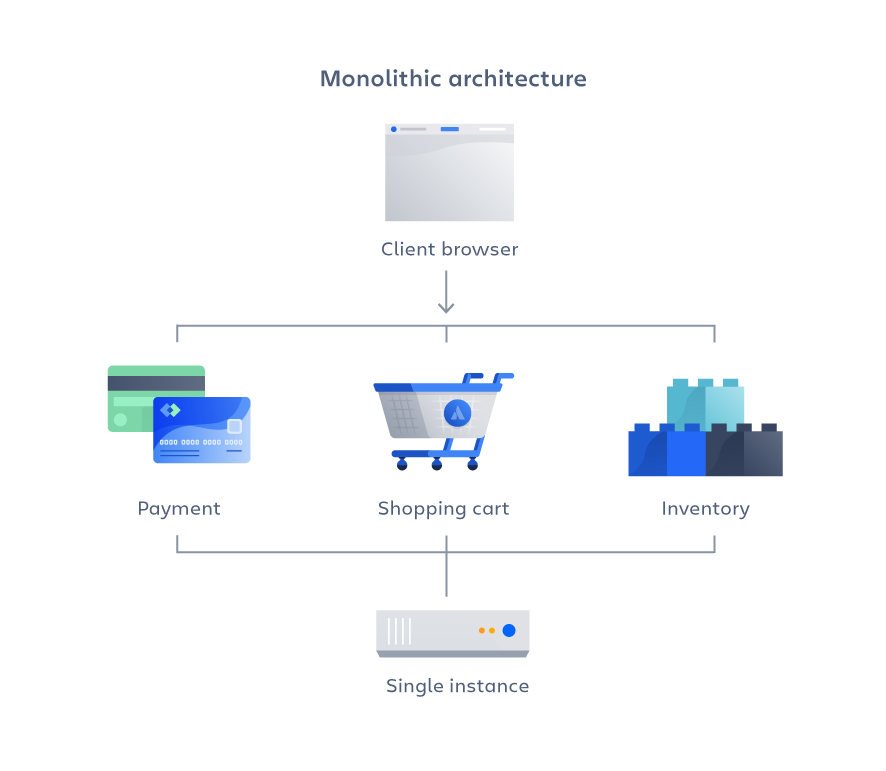
\includegraphics[width=\linewidth]{img/cap2/Monolithic_architecture.png}
		\end{subfigure}
		\begin{subfigure}{0.5\textwidth}
			\centering
			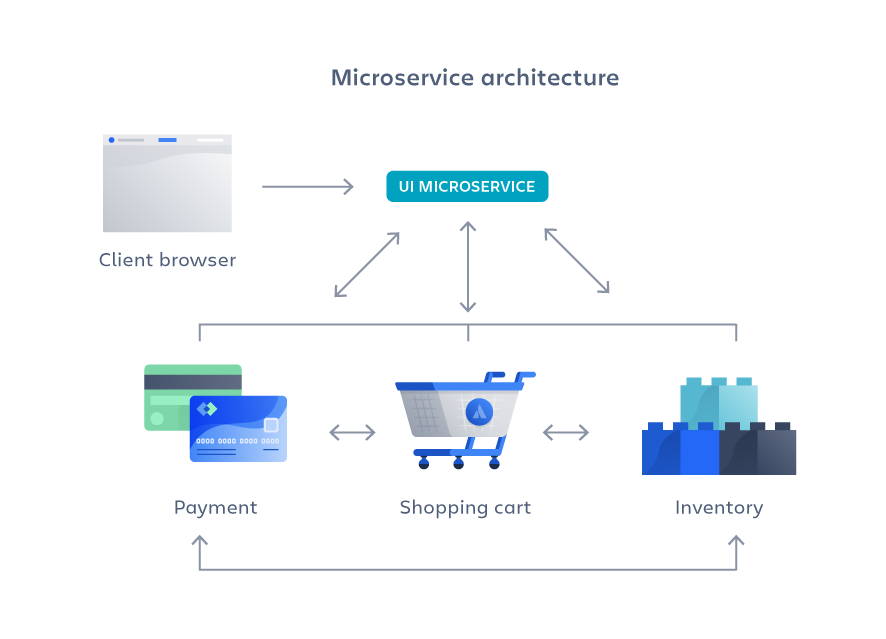
\includegraphics[width=\linewidth]{img/cap2/Microservice_architecture.png}
		\end{subfigure}
		\caption{Principio di funzionamento di un'applicazione monolitica e una a microservizi\cite{site:archComparison} }
	\end{figure}
	
	
	
\section{Deployment tradizionale}

	La metodologia tradizionale di deployment prevede l'esecuzione delle applicazioni direttamente sul server fisico.
	Sebbene semplice ed immediato questo modo di procedere non è ottimale, non permette infatti di scalare l'applicazione ponendo dei limiti sull'utilizzo di risorse (CPU, RAM, disco,\dots) e si corre il rischio che una seconda applicazione non riesca a garantire le prestazioni desiderate.
	Si potrebbe cercare un'alternativa a questo problema eseguendo ogni applicazione su un server fisico distinto, ma anche una tale soluzione non è adatta a un contesto reale risultando molto costosa e portando a un sottoutilizzo delle risorse complessive\cite{doc:kube}.



\section{Deployment su macchine virtuali}

	Le macchine virtuali sono pacchetti software piuttosto pesanti, in grado di eseguire l'emulazione dei dispositivi hardware di basso livello quali CPU, RAM, dischi e schede di rete.
	Il deployment su macchine virtuali (anche chiamato deployment virtualizzato) prevede l'esecuzione di più macchine virtuali sul server fisico, ciascuna delle quali esegue un sistema operativo che a sua volta esegue una o più applicazioni.
	Un simile approccio è in grado di far fronte ad alcune delle problematiche del deployment tradizionale:
	
	\begin{itemize}
		\item \emph{Limitazione delle risorse:}
			In funzione di quanto detto sopra è possibile limitare le risorse dedicate ad una macchina virtuale in termini di tempo di CPU, quantità di RAM, etc.
		\item \emph{Isolamento:}
			Le macchine virtuali vengono eseguite in un ambiente isolato e completamente autonomo che le rende immuni da tentativi di interferenza da parte di altre macchine virtuali attive sullo stesso host.
	\end{itemize}
	
	Contrariamente, i principali svantaggi delle macchine virtuali riguardano la ridotta velocità di generazione e distribuzione delle stesse e il maggiore spazio di archiviazione richiesto:
	trattandosi di \emph{immagini} di un sistema indipendente possono infatti richiedere diverso tempo per essere generate e configurate, l'affiancamento di diverse macchine virtuali porta inoltre alla duplicazione del sistema operativo installato su di esse, con un conseguente utilizzo di spazio di archiviazione.



\section{Deployment su container}
	
	\label{sec:depl_on_cont}
	Un \emph{container} è un modello di virtualizzazione più leggero rispetto ad una macchina virtuale che racchiude un software e tutte le dipendenze necessarie ad eseguirlo.
	Al pari delle macchine virtuali i container rappresentano un ambiente isolato, con risorse limitate ed un proprio file system per l'esecuzione del software ma non virtualizzano un intero sistema operativo.
	L'uso di container offre una grande efficienza in fase di sviluppo  e di esecuzione, contengono infatti solo software di alto livello e sono molto veloci da modificare, oltre al fatto che non dovendo virtualizzare un sistema operativo la loro esecuzione risulta molto più rapida e meno esosa di risorse hardware.
	Per finire molti sistemi runtime per container mettono a disposizione degli sviluppatori repository pubbliche con immagini preconfezionate di software popolari, il tutto al fine di avere uno sviluppo ancora più rapido
	\cite{doc:kube, site:container_vs_VM}.
	
	\begin{figure}[tbp]
		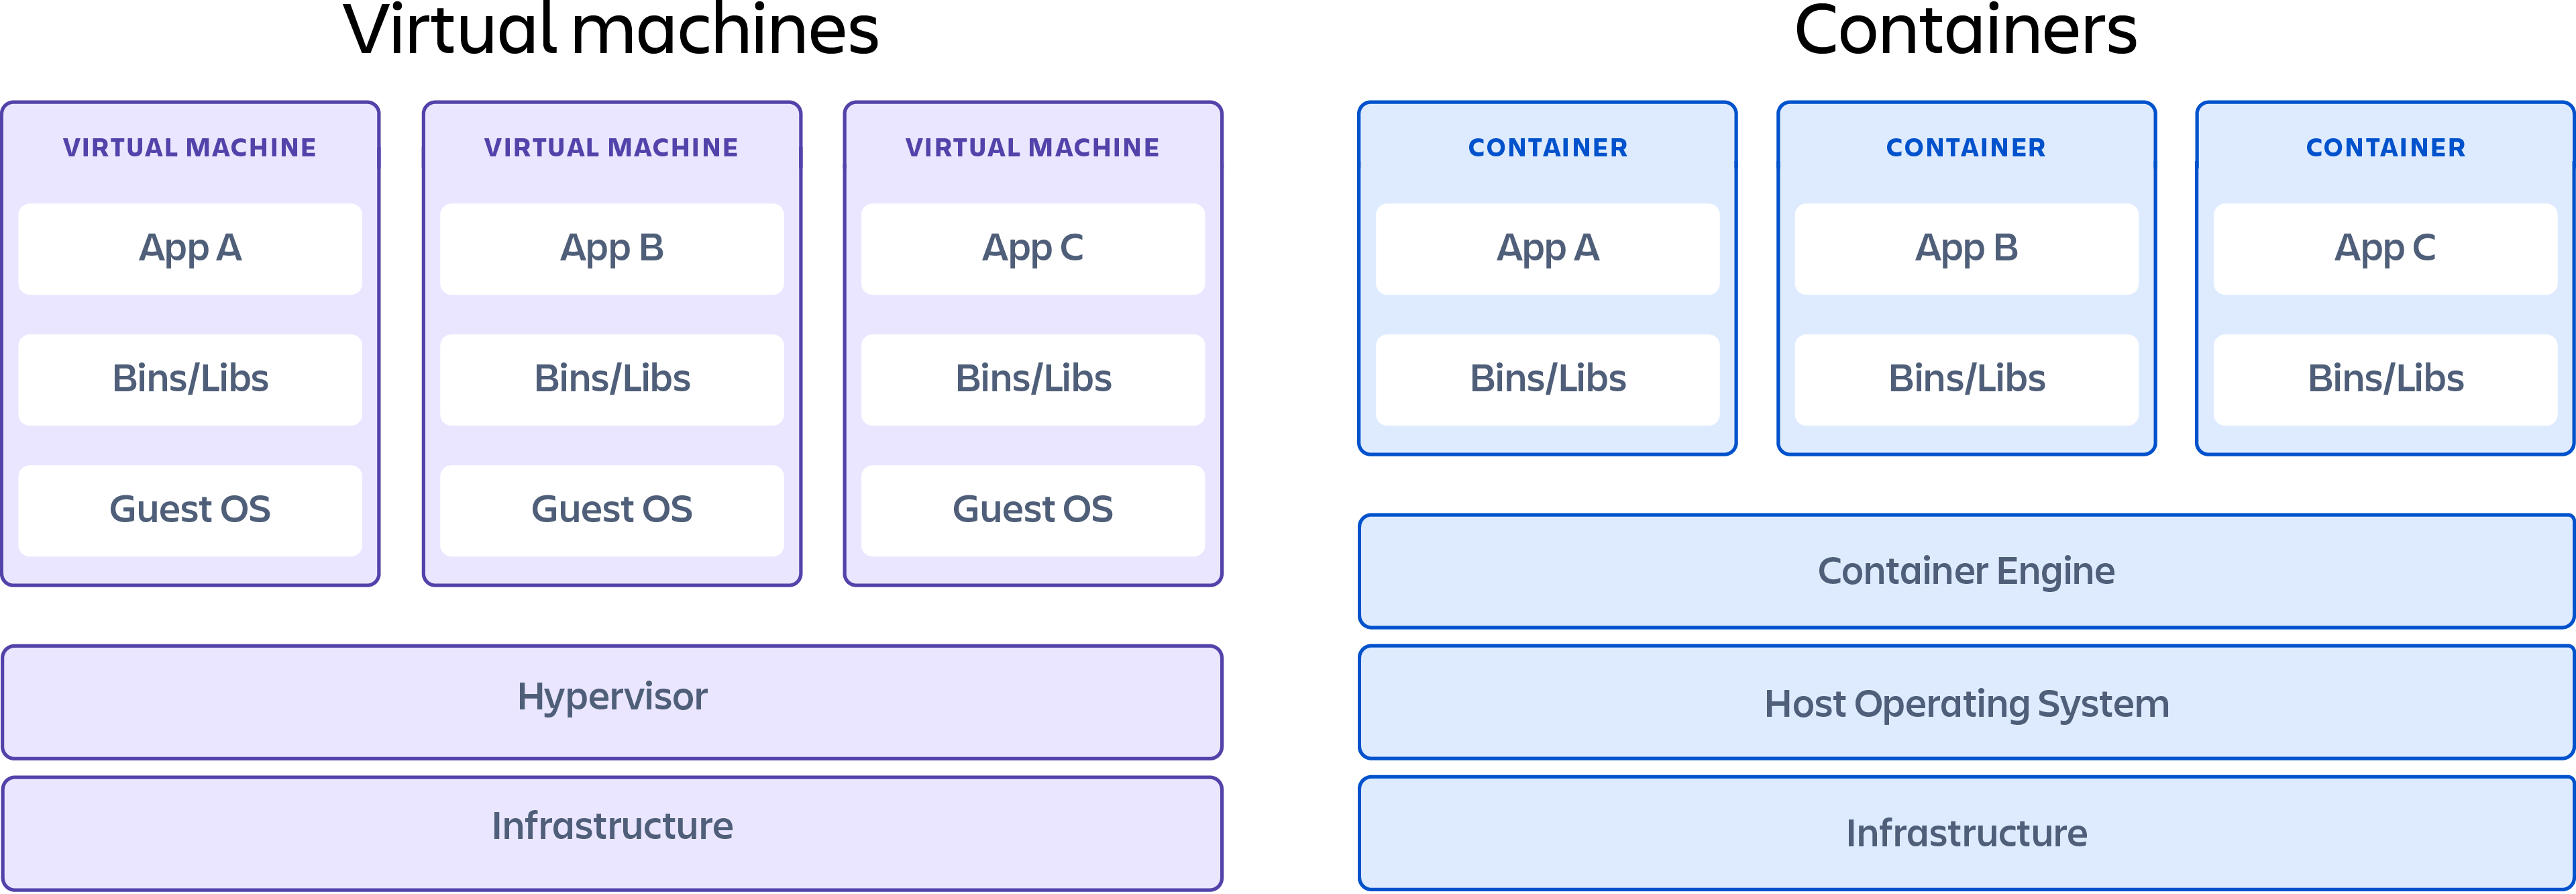
\includegraphics[width=\textwidth]{img/cap2/Diagram_Containers_VirtualMachines.png}
		\caption{Confronto tra un sistema basato su macchine virtuali e container\cite{site:container_vs_VM}}
		\label{fig:VM_vs_container}
	\end{figure}











	\chapter{Architettura del sistema}

	Nel corso di questo capito verrà dapprima posta l'attenzione sulla struttura dei due sistemi sviluppati, per poi focalizzarsi sulla descrizione delle tecnologie utilizzate.


\section{Struttura}
	
	Come già precedentemente evidenziato il sistema è stato sviluppato seguendo due filosofie di sviluppo differenti, dapprima secondo un approccio monolitico ed in seguito seguendo un approccio a microservizi;
	le due applicazioni sono tra di loro molto simili, condividono buona parte del codice e sfruttano le stesse tecnologie.
	
	\smallskip
	L'applicazione sviluppata in modo monolitico espone alcune chiamate API REST, che tramite il protocollo HTTP le permettono di ricevere richieste ed inviare risposte agli applicativi lato client.
	Lo scambio di informazioni tra client e server avviene scambiando messaggi in formato JSON ed è protetto con algoritmi di crittografia e metodi di autenticazione tramite token, il tutto per garantire sicurezza e privatezza dei dati scambiati.
	Per la conservazione dei dati persistenti ()quali informazioni sugli utenti, sulla merce in magazzino o sugli ordini) si utilizza infine un database PostgreSQL.
	
	\smallskip
	L'applicazione a microservizi nasce dall'applicazione monolitica e la scompone in un numero di unità pari al numero di servizi complessivamente offerti, nel contesto applicativo ciascun modulo si riduce così ad esporre una singola chiamata API, occupandosi di un singolo aspetto tra i passi successivi che portano dalla scelta dei prodotti fino alla spedizione dell'ordine.
	Il sistema si compone in questo caso di un cluster di server eseguiti all'interno di container e, in un contesto più ampio, di un cluster Kubernetes.



\section{Tecnologie utilizzate}

\subsection{Python}
	
	Python è un linguaggio di programmazione \emph{general-purpose} orientato agli oggetti e ad alto livello, molto diffuso in ambiti quali l'analisi dei dati, l'intelligenza artificiale, la finanza e la sicurezza informatica\cite[7-8]{book:lutz-python}.
	Pone grande enfasi sulla leggibilità e dispone di una sintassi particolarmente semplice che, insieme a una vastissima gamma di librerie, permette una grande riduzione in termini di linee di codice\cite{wiki:python}.
	
	
\subsection{PostgreSQL}
	
	PostgreSQL è un Database Management System (DBMS) di tipo relazionale e ad oggetti, molto potente ed open source.
	Si tratta di una valida alternativa ad altri progetti sia liberi che con licenza ed è divenuto celebre nel tempo per alcuni suoi punti di forza quali la programmabilità, la quale permette di incrementare astrazione, affidabilità e prestazioni\cite{doc:postgresql, wiki:postgresql}.


\subsection{Docker}
	
	Docker è una piattaforma aperta per lo sviluppo, la consegna e l'esecuzione di applicazioni all'interno di container.
	All'interno di Docker sono definiti essenzialmente due oggetti principali:
	
	\begin{description}
		\item[Immagini]
			Un immagine è un template di sola lettura contenente le istruzioni per generare un nuovo container.
			La generazione di nuove immagini è estremamente semplice ed avviene sulla base di istruzioni definite in un \emph{Dockerfile}, un file contenente le istruzioni per la generazione di un ambiente preconfigurato e pronto per l'esecuzione.
			Ogni istruzione all'interno del Dockerfile corrisponde a un livello nella generazione dell'immagine, facilitando la condivisione e la distribuzione della stessa; quando un Dockerfile viene modificato e l'immagine è ricompilata, solo i livelli che hanno subito modifiche vengono ricompilati.
			Si tratta quindi di strutture molto leggere, piccole e veloci se comparate ad altri modelli di virtualizzazione\cite{doc:docker-overview}.
			
		\item[Container]
			L'idea alla base dei container è già stata spiegata nella Sezione \ref{sec:depl_on_cont},
			nel contesto di Docker i container assumono il ruolo di istanze eseguibili delle immagini\cite{doc:docker-overview}.
	\end{description}
	
	Docker risulta ottimo per la gestione di container su un singolo host, offrendo strumenti per la limitazione e il monitoraggio delle risorse o il bilanciamento del carico (attraverso \emph{Docker Swarm} o \emph{Overlay Network Driver}), con caratteristiche che risultano tuttavia limitate rispetto ad altri orchestratori più avanzati\cite{site:kube_better_docker}.
	
	
\subsection{Kubernetes}
	
	Kubernetes è una piattaforma open source per l'automazione della distribuzione, scalabilità e gestione di applicazioni eseguite su container, azioni che nell'insieme prendono il nome di \emph{orchestrazione}.
	La necessità di orchestratori di container nasce in ambito di produzione, laddove c'è la necessità di gestire un gran numero di container ed assicurarsi che i servizi offerti siano sempre attivi\cite{doc:docker-overview}.

	Alcune delle caratteristiche principali di Kubernetes sono:
	\begin{description}
		\item[Gestione delle risorse]
			Permette di porre limiti sulle risorse utilizzabili da un container (RAM, CPU, disco, etc.).
		
		\item[Bilanciamento del carico]
			\`E in grado di gestire più repliche di uno stesso container e gestire il traffico in ingresso distribuendolo uniformemente sulle istanze attive.
			Fornisce inoltre la funzione di \emph{auto-scaling} che permette di variare il dinamicamente il numero di istanze di un container sulla base del traffico di rete.
			
		\item[Self-healing]
			Termina automaticamente i container che si sono bloccati e li sostituisce con nuove istanze degli stessi.
			
		\item[Configurazione dichiarativa]
			\`E possibile lavorare in modalità DSC (\emph{Desired State Configuration}), in cui un cluster può essere configurato utilizzando dei file che descrivono lo stato in cui si vuole portare il sistema.
			La fase di transizione dallo stato attuale del cluster allo stato desiderato è del tutto trasparente all'utente e non è in alcun modo modificabile dall'utente, sarà Kubernetes a prendere tutte le decisioni al fine di raggiungere lo stato finale.
	\end{description}
	
	Gli elementi chiave di Kubernetes sono \emph{Nodi}, \emph{Cluster}, \emph{Pod}, \emph{Deployment}, \emph{Service}.
	Di seguito una breve presentazione per ognuno di essi:
	
	
\paragraph{Cluster}
	Un cluster è l'unita logica più ampia definita in Kubernetes e rappresenta l'ambiente all'interno del quale sono orchestrati i container.
	
	
\paragraph{Nodi}
	I nodi possono essere una macchina fisica o virtuale e rappresentano i punti tra i quali viene suddiviso il carico di lavoro.
	Ne sono definiti due tipi: i \emph{control plane node} e i \emph{worker node}, i primi gestiscono l'interazione con il cluster e si occupano di distribuire uniformemente il carico di lavoro tra i \emph{worker node}; i secondi sono nodi operativi, sui quali vengono istanziati i \emph{pod}\cite{doc:kube-nodes}.


\paragraph{Pod}
	Un Pod è la più piccola unità definibile con Kubernetes e corrisponde a un gruppo di uno o più container che condividono spazio di archiviazione e risorse di rete.
	Ogni pod modella di fatto un host logico\cite{doc:kube-pod}.


\paragraph{Deployment e Replicaset}
	Un \emph{Deployment} è un oggetto Kubernetes che permette di dichiarare come le applicazioni al suo interno debbano essere gestite, distribuite e quante risorse gli si debba dedicare.
	All'interno del deployment viene solitamente definito un oggetto \emph{ReplicaSet}, il quale racchiude un insieme di pod che condividono una configurazione comune.
	La risorsa \emph{ReplicaSet} si occupa di mantenere il numero di repliche desiderato per ciascun pod, istanziandone di nuovi o distruggendo quelli bloccati.


\paragraph{Service}

	
	
\subsection{API REST}
	
	
	
	
\subsection{JWT}
	
	
	
	
	
	
	
	
	
	
	
	
	
	
	
	
	
	
	
	
	
	
	
	
	
	
	
	
	
	
	
	
	
	
	
	
	
	
	
	
	
	
	
	
	
	
	
	
	
	\chapter{Implementazione}

	Le due applicazioni sviluppate mirano a soddisfare le stesse richieste e presentano perciò una similarità molto stretta a livello di tecnologie utilizzate.
	Nel corso di questo capitolo verrà presentata dapprima l'applicazione monolitica, analizzandone i servizi offerti, la struttura interna e le scelte progettuali compiute;
	in seguito si passerà all'analisi del sistema a microservizi, concentrandosi sul processo di decomposizione del problema generale.
	
	L'applicazione espone complessivamente 5 servizi
	
	\begin{enumerate}
		\item \emph{Autenticazione}:
			Autentica gli utenti e verifica la validità dei token presentati.
		
		\item \emph{Gestione clienti}:
			Permette la registrazione di nuovi clienti.
			
		\item \emph{Gestione ordini}:
			Permette la generazione di nuovi ordini.
			
		\item \emph{Gestione pagamenti}:
			Gestisce il pagamento degli ordini.
			
		\item \emph{Spedizioni}:
			Permette di generare nuove spedizioni e verificare lo stato di una spedizione esistente.
	\end{enumerate}
	

\section{Autenticazione e autorizzazione}

	Gli utenti devono poter compiere solo le operazioni per le quali sono autorizzati sulla base del proprio tipo di utente, un cliente non deve per esempio poter rifornire il magazzino.
	Per questo motivo ad ogni richiesta inviata tramite API viene aggiunto un token JWT con quattro \emph{claim} privati: \texttt{badge\_n}, il numero di tessera del cliente, \texttt{created}, data e ora di creazione, \texttt{expires}, data e ora di scadenza, \texttt{role}, tipologia di utente.
	
	Il token è rilasciato durante la fase di login ed ha una validità di trenta minuti, superata la quale occorre autenticarsi nuovamente.
	Il processo di login segue i seguenti passi:
	
	\begin{enumerate}
		\item L'applicazione riceve una richiesta POST sul percorso \texttt{/login} in cui sono forniti email e hash della password (generato secondo l'algoritmo SHA-3) dell'utente che richiede di autenticarsi.
		
		\item Viene interrogato il database e vengono recuperate le informazioni associate all'utente sulla base dell'email fornita.
		
		\item Se lo hash presente nel database e quello fornito coincidono, viene generato il token inserendo tutti i claim sopra elencati.
		
		\item Il token viene firmato e restituito al client.
	\end{enumerate}
	
	Il token è firmato utilizzando l'algoritmo a chiave segreta HS256, procedura fondamentale al fine di garantire l'autenticità del token stesso quando questo sarà ripresentato.
	
	
\section{Database}

	Il database si compone di sei tabelle (vedi Figura \ref{fig:dbSchema}):
	
	\begin{itemize}
		\item \emph{Articles}: modella il magazzino, contiene i prodotti e le relative quantità.
			\begin{itemize}
				\item \emph{barcode}: codice a barre univoco dell'articolo;
				\item \emph{name}: nome dell'articolo;
				\item \emph{quantity}: quantità presente in magazzino;
				\item \emph{unit\_price}: costo unitario del prodotto.
			\end{itemize}
			Per la colonna \emph{quantity} si è definito il vincolo \texttt{positive\_quantity\_remaining\_check}, il quale impedisce che la quantità residua di un prodotto assuma valori negativi.
			\label{sec:quantityCheck}
		
		\item \emph{Customers}: elenco dei clienti registrati.
			\begin{itemize}
				\item \emph{customerid}: id univoco dell'utente;
				\item \emph{surname}: cognome;
				\item \emph{badge\_n}: numero di tessera;
				\item \emph{sex}: sesso;
				\item \emph{dob}: data di nascita;
				\item \emph{email}: email;
				\item \emph{password\_hash}: codice hash della password;
				\item \emph{customerrole}: tipologia di utente (vedi tabella successiva).
			\end{itemize}
			
		\item \emph{OrderItems}: contiene gli articoli acquistati in ogni ordine.
			\begin{itemize}
				\item \emph{articleid}: codice a barre dell'articolo acquistato;
				\item \emph{orderid}: id dell'ordine in cui è stato acquistato l'articolo;
				\item \emph{quantity}: quantità acquistata.
			\end{itemize}
			
		\item \emph{Orders}: contiene gli ordini effettuati.
			\begin{itemize}
				\item \emph{orderid}: id univoco dell'ordine;
				\item \emph{badge\_n}: numero di tessera del cliente che ha effettuato l'ordine;
				\item \emph{orderdate}: data ed ora in cui è stato generato l'ordine;
				\item \emph{total\_price}: prezzo complessivo dell'ordine;
				\item \emph{orderstate}: stato dell'ordine (vedi tabella successiva).
			\end{itemize}
			
		\item \emph{orderstate}: contiene gli stati definiti per un ordine.
			Essi sono rappresentati in una tabella a parte al fine di garantire coerenza nel database e facilità di comprensione e manutenzione.
			\begin{itemize}
				\item \emph{id}: numero intero associato allo stato;
				\item \emph{statename}: nome dello stato;
			\end{itemize}
			
		\item \emph{Roles}: contiene i ruoli definiti per gli utenti.
			Valgono le stesse considerazioni fatte per la tabella precedente.
			\begin{itemize}
				\item \emph{rolename}: nome del ruolo
			\end{itemize}
		
	\end{itemize}
	
	\begin{figure}[tbp]
		\centering
		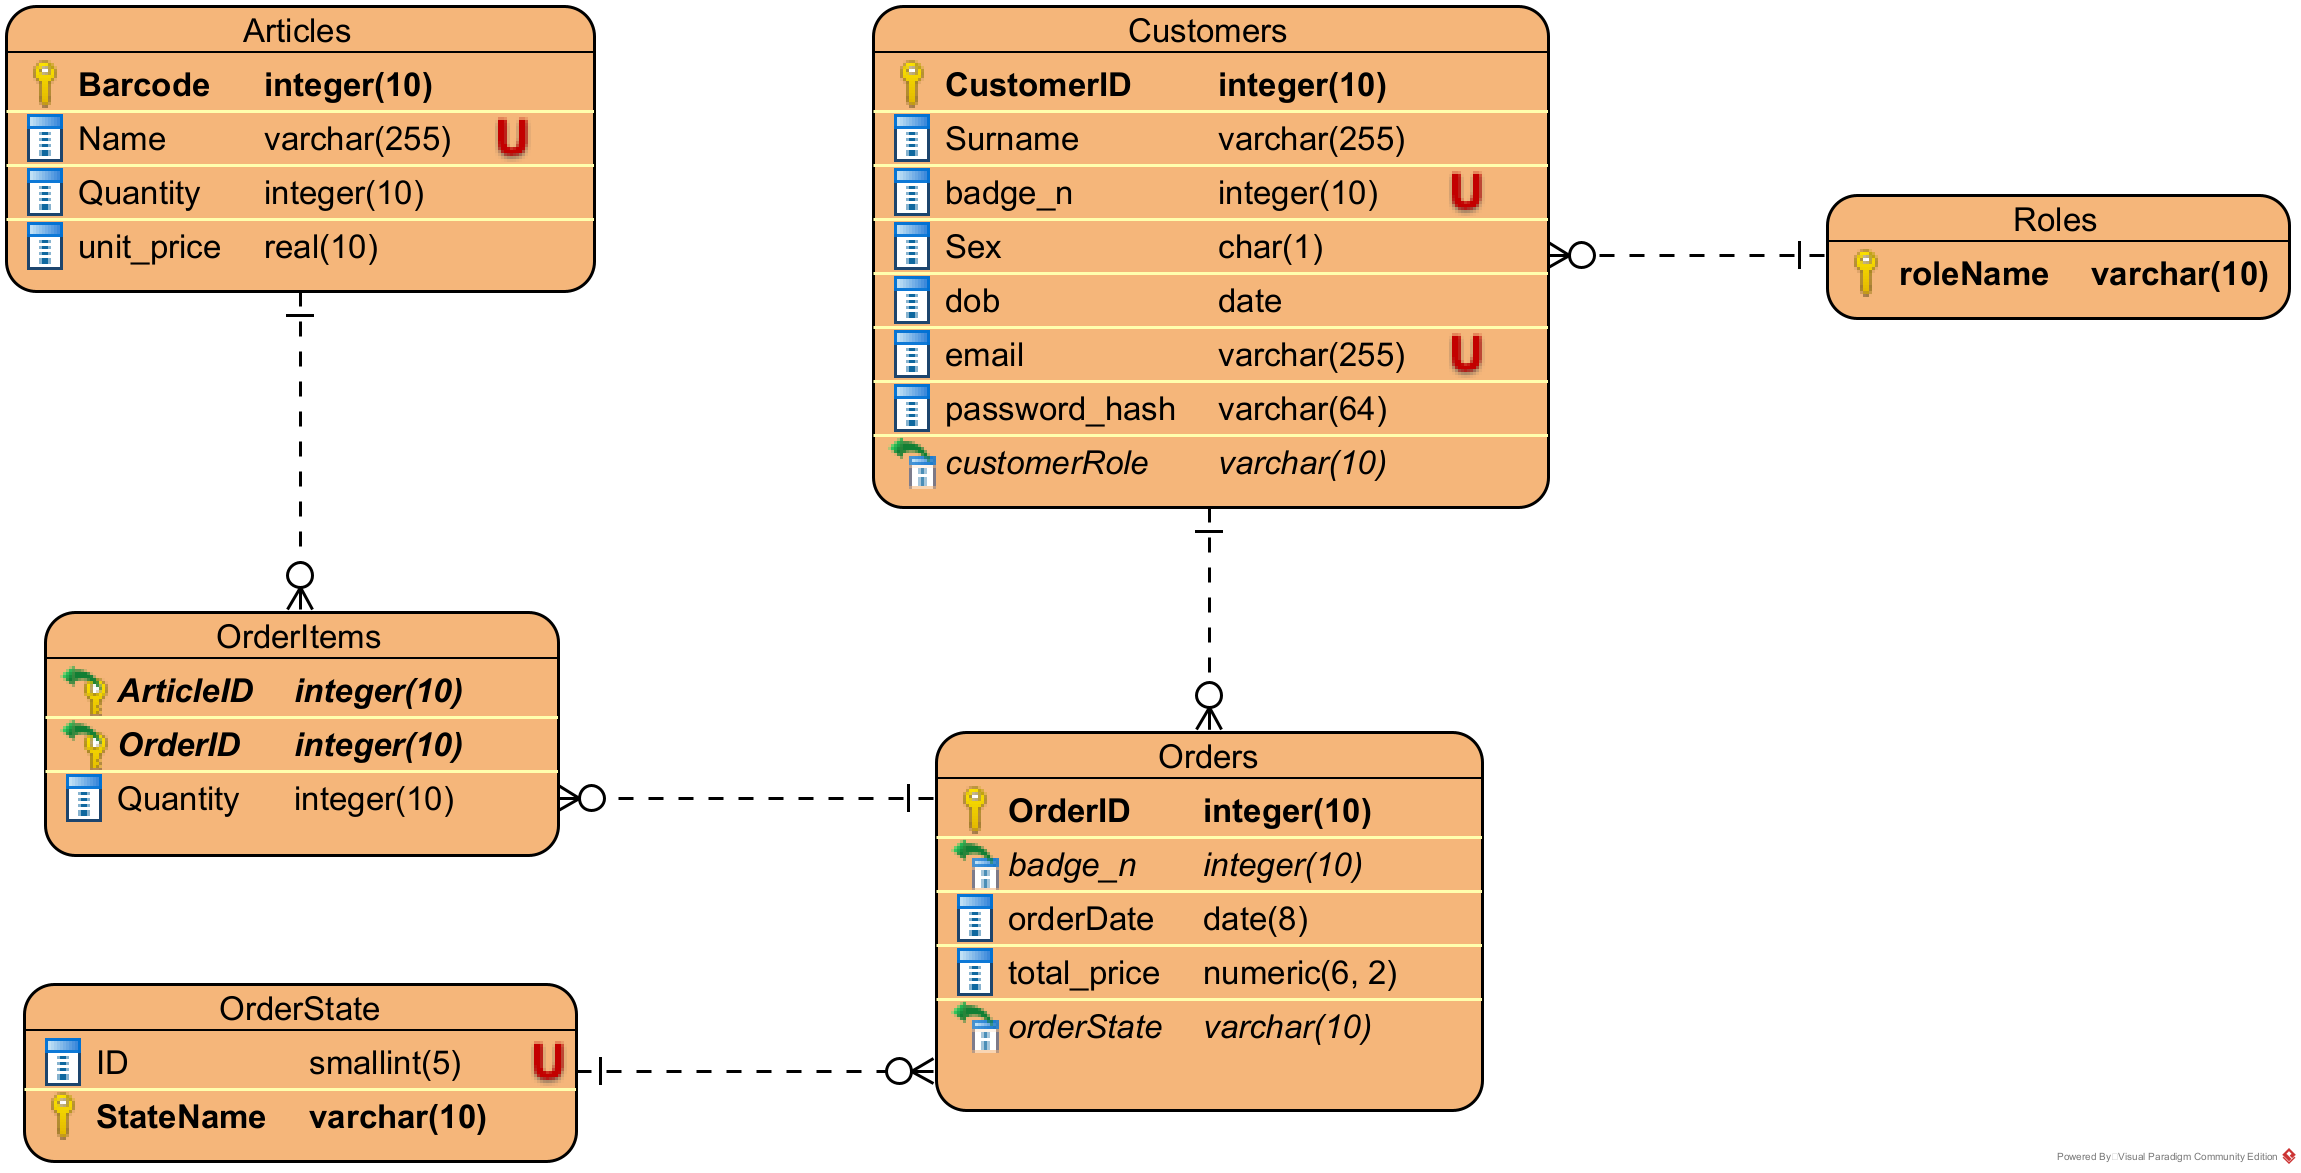
\includegraphics[width=\textwidth]{img/cap4/ER-Diagram.png}
		\caption{Schema del database}
		\label{fig:dbSchema}
	\end{figure}
	
	
\section{Esecuzione delle richieste}

	Le richieste ricevute sono eseguite nel seguente modo:
	
	\begin{enumerate}
		\item Vengono verificati la validità del token fornito e i permessi dell'utente ad effettuare la richiesta, se uno di questi due controlli fallisce viene inviata direttamente una risposta di errore.
		
		\item La gestione della richiesta viene demandata alla classe specifica, che interroga il database se necessario e predispone un oggetto JSON di risposta.
		Ogni classe dispone dei permessi in scrittura sul database, si è compiuta questa scelta al fine di evitare i colli di bottiglia tipici di una gestione centralizzata.
		
		\item Viene generata la risposta, restituendo la risorsa richiesta in formato JSON insieme a un codice di stato (\emph{status code}).
		Il codice di stato è utile per identificare l'esito positivo o negativo della richiesta, inserendo eventualmente l'errore all'interno di una macro categoria.
	\end{enumerate}
	
	

\section{Evoluzione dello stato di un ordine}
	
	Sono definiti sei stati in cui può trovarsi un ordine, si riporta il diagramma a stati finiti in Figura \ref{fig:diagStatoOrdine}.
	
	\begin{itemize}
		\item \emph{Created}: L'ordine è stato ricevuto.
		\item \emph{Confirmed}: L'ordine può essere soddisfatto, i prodotti acquistati sono stati registrati.
		\item \emph{Cancelled}: Non è possibile soddisfare l'ordine, almeno un prodotto è presente a magazzino in quantità insufficiente.
		\item \emph{Paid}: \`E stato ricevuto il pagamento.
		\item \emph{Refused}: Il pagamento è stato rifiutato.
		\item \emph{OnDelivery}: L'ordine è stato spedito.
	\end{itemize}
	
	\begin{figure}[tbp]
		\centering
		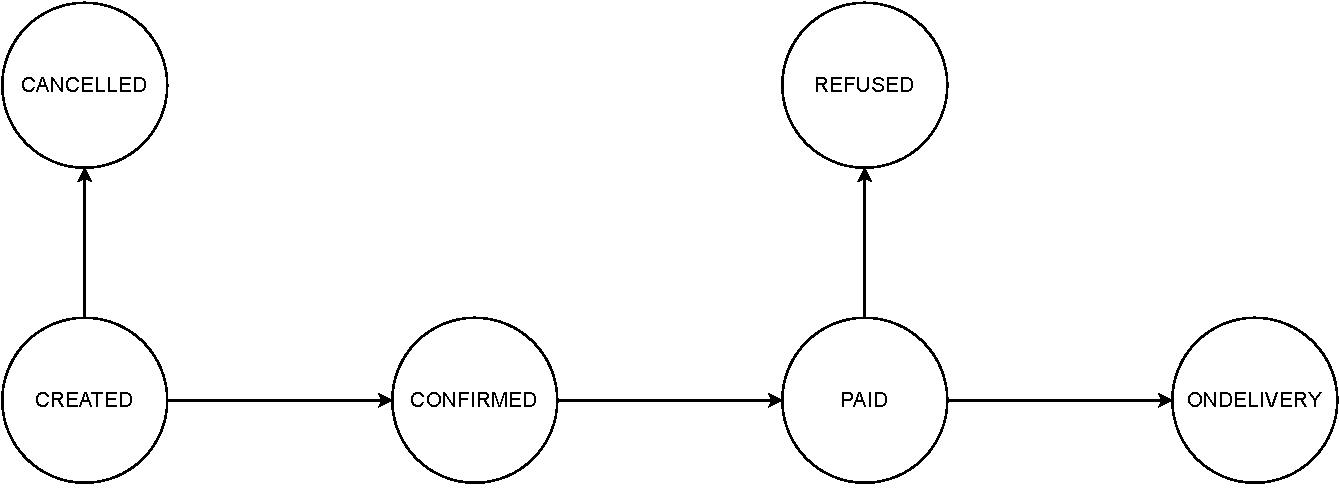
\includegraphics[width=0.9\textwidth]{img/cap4/statiOrdine.pdf}
		\caption{Diagramma a stati finiti degli stati definiti per un ordine}
		\label{fig:diagStatoOrdine}
	\end{figure}
	
	Il processo di creazione di un nuovo ordine ha inizio con l'arrivo di una richiesta POST all'API sul percorso \texttt{/newOrder} e può essere effettuato solamente da utenti di tipo \emph{customer}.
	Il corpo della richiesta deve essere in formato JSON e contenere un array di prodotti selezionati e la relativa quantità;
	la struttura deve essere quella riportata nel Codice \ref{lst:json_newOrder}.
	
	\begin{listing}[tb]
		\inputminted{json}{codici/cap4/nuovoOrdine.json}
		\caption{Struttura del corpo della richiesta per la creazione di un nuovo ordine}
		\label{lst:json_newOrder}
	\end{listing}
	
	Non è necessario specificare l'identificativo dell'utente, in quanto questa informazione, insieme al tipo di utente, è già presente all'interno del token ed è recuperata automaticamente.
	I passaggi successivi riguardano:
	
	\begin{enumerate}
		\item Viene registrato il nuovo ordine nella tabella \emph{Orders} del database, il quale si occupa di assegnare un id univoco.
		Lo stato dell'ordine è impostato su \emph{created} finché non ha l'id assegnato e viene in seguito modificato in \emph{created}.
		
		\item Vengono prelevati i prodotti ordinati dal magazzino, modificando le quantità residue nella tabella \emph{Articles}.
		Se si tenta di rimuovere un numero di prodotti superiore a quelli residui presenti in magazzino viene generata un'eccezione per la violazione del \emph{vincolo check} spiegato alla Sezione \ref{sec:quantityCheck};
		il database esegue il rollback e lo stato dell'ordine è impostato su \emph{Cancelled}.
		
		\item Vengono registrati tutti i prodotti ordinati con la quantità associata nella tabella \emph{OrderItems} del database.
		
		\item Viene calcolato il prezzo finale dell'ordine e memorizzato nella tabella \emph{Orders}.
	\end{enumerate}
	
	Se tutto va a buon fine all'utente viene comunicata la somma da pagare e lo stato dell'ordine è modificato in \emph{Confirmed}.
	

	
\section{Implementazione dei microservizi}

	L'applicazione a microservizi nasce dal codice dell'applicazione monolitica, ma lo riorganizza in unità indipendenti sulla base dei diversi servizi offerti.
	Al fine di evitare colli di bottiglia dovuti alla presenza di un singolo punto d'ingresso per le richieste, ogni microservizio espone delle proprie API.
	
	\begin{figure}[tbp]
		\centering
		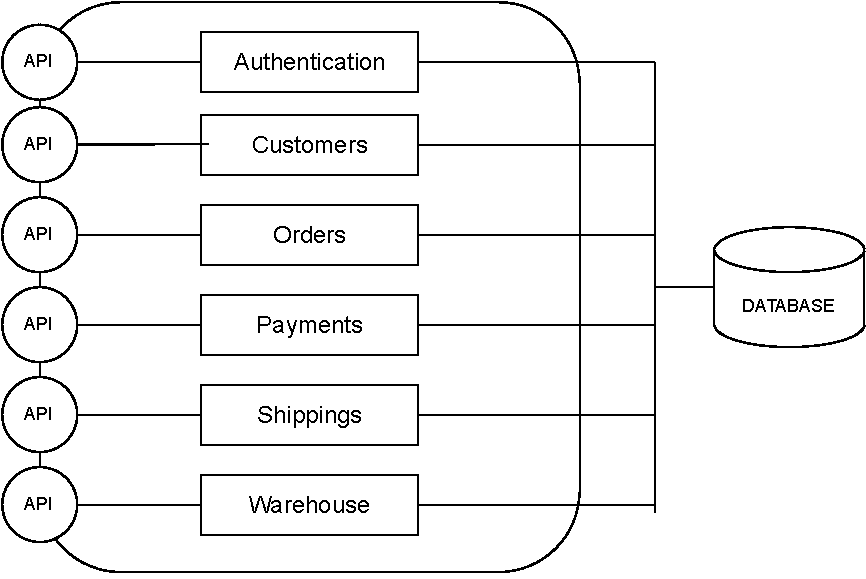
\includegraphics[height=0.5\textwidth]{img/cap4/microservizi.pdf}
		\caption{Struttura del sistema a microservizi}
		\label{fig:microservizi}
	\end{figure}
	
	Sono stati sviluppati sei microservizi, uno schema generale del sistema è mostrato in Figura \ref{fig:microservizi}:
	
	\begin{itemize}
		\item \emph{Authentication}:
			Gestisce l'autenticazione dell'utente e controlla la validità dei token.
			Espone API con metodo POST sul percorso \texttt{/login} alla porta 5000.
		
		\item \emph{Customers}:
			Permette l'iscrizione di nuovi utenti, tramite una API con metodo POST alla porta 5005 sul percorso \texttt{/registerCustomer}.
		
		\item \emph{Orders}:
			Gestisce il processo di creazione di un nuovo ordine.
			Espone API con metodo POST alla porta 5002 sul percorso \texttt{/newOrder}.
		
		\item \emph{Payments}:
			Gestisce la procedura di pagamento.
			Espone API con metodo POST alla porta 5003 sul percorso \texttt{/payOrder}	
		
		\item \emph{Shippings}:
			Genera nuove spedizioni e permette di controllare lo stato di una spedizione.
			Espone API con metodo POST alla porta 5004 sul percorso \texttt{/trackOrder}
		
		\item \emph{Warehouse}:
			Gestisce il magazzino.
			Ha una propria API attiva sulla porta 5001 al percorso \texttt{productsList}, con metodo GET per richiedere la lista dei prodotti presenti in magazzino, POST per caricare nuovi prodotti.
		
	\end{itemize}

























	
	
	\chapter{Risultati ottenuti}

	Il sistema è stato avviato in locale, su un computer che funge sia da nodo \emph{master} che da nodo \emph{worker}.
	Al fine di analizzare le performance dei due sistemi (monolitico e a microservizi) è stato realizzato uno script che effettua mille ordini in successione.
	Le operazioni eseguite nel dettaglio sono le seguenti:
	
	\begin{enumerate}
		\item Viene selezionato in modo casuale un utente con il quale si effettua il login.
		
		\item Viene richiesta la lista articoli disponibili.
			Dalla lista vengono selezionati alcuni prodotti in modo casuale (da 1 a 15 prodotti diversi), ciascuno in quantità casuale tra 1 e 10;
			si genera così un carrello virtuale.
			
		\item Viene inviato l'ordine con i prodotti scelti.
		
		\item L'ordine viene pagato.
		
		\item Se non si sono generati errori la procedura è completata e si passa all'esecuzione della prossima iterazione.
	\end{enumerate}
	
	Ad ogni iterazione lo script memorizza l'intervallo di tempo in sei differenti punti:
	
	\begin{enumerate}
		\item Inizio della nuova iterazione.
		
		\item Completato il login dell'utente.
		
		\item Ottenuta la lista di prodotti dal server.
		
		\item Carrello riempito con i prodotti selezionati secondo la modalità precedentemente descritta.
		
		\item Il nuovo ordine è stato generato.
		
		\item Fine.
	\end{enumerate}
	
	Si possono quindi calcolare cinque intervalli di tempo, indicati in ordine con lettere da A ad E.
	In Tabella \ref{tab:tempi-monolitica} e \ref{tab:tempi-microserv} sono riportati gli indici statistici più rilevanti ottenuti dai dati inerenti i tempi di esecuzione di ogni fase, in Figura \ref{fig:grafici-monolitica} e \ref{fig:grafici-microserv} i dati sono invece rappresentati sotto forma di boxplot ed istogramma.

	L'indice di maggior interesse è sicuramente la media e si nota un generale leggero vantaggio per l'applicazione monolitica, dovuto al \emph{overhead} introdotto dall'orchestratore dei container.
	In un'applicazione molto semplice come quelle realizzate per questa ricerca la differenza è poco marcata o addirittura a
	Va anche tenuto in considerazione che il test è stato eseguito su un personal computer di potenza limitata, sicuramente ben lontano dalla capacità di calcolo offerta da un server reale.





	\begin{table}[tbp]
		\[
		\begin{array}{lccccc}
			\toprule
			\mbox{\textbf{Fase}} & \textbf{A} & \textbf{B} & \textbf{C} & \textbf{D} & \textbf{E}\\
			\midrule
			\mbox{Media} & 43.64 & 42.21 & 0.05 & 49.53 & 64.13\\
			\mbox{Minimo} & 29.74 & 30.36 & 0 & 35.69 & 30.81\\
			\mbox{1° quartile} & 38.23 & 37.44 & 0 & 43.62 & 37.0\\
			\mbox{Mediana} & 40.38 & 39.29 & 0 & 45.93 & 39.29\\
			\mbox{3° quartile} & 42.93 & 41.28 & 0 & 48.31 & 44.07\\
			\mbox{Massimo} & 208.61 & 170.06 & 1.54 & 179.83 & 271.9\\
			\bottomrule
		\end{array}
		\]
		\caption{Valori statistici ottenuti dall'esecuzione dell'applicazione monolitica. Tempi espressi in ms}
		\label{tab:tempi-monolitica}
	\end{table}
	
	\begin{table}[tbp]
		\[
		\begin{array}{lccccc}
			\toprule
			\mbox{\textbf{Fase}} & \textbf{A} & \textbf{B} & \textbf{C} & \textbf{D} & \textbf{E}\\
			\midrule
			\mbox{Media} & 44.06 & 44.15 & 0.06 & 62.84 & 7.64\\
			\mbox{Minimo} & 34.14 & 34.36 & 0 & 46.38 & 5.35\\
			\mbox{1° quartile} & 37.78 & 37.41 & 0 & 53.26 & 6.97\\
			\mbox{Mediana} & 39.3 & 38.86 & 0 & 56.49 & 7.35\\
			\mbox{3° quartile} & 41.45 & 40.97 & 0 & 60.51 & 8.02\\
			\mbox{Massimo} & 170.22 & 186.01 & 0.69 & 201.11 & 35.31\\
			\bottomrule
		\end{array}
		\]
		\caption{Valori statistici ottenuti dall'esecuzione dell'applicazione a microservizi. Tempi espressi in ms}
		\label{tab:tempi-microserv}
	\end{table}

	\begin{figure}[tbp]
		\begin{subfigure}{0.5\textwidth}
			\centering
			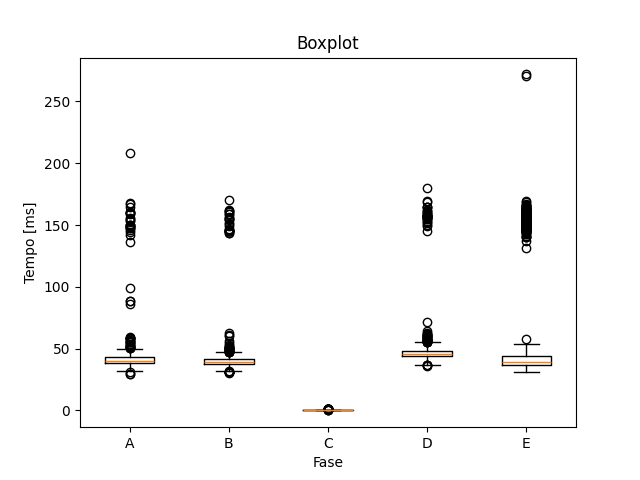
\includegraphics[width=\linewidth]{img/cap5/monolithic/boxplot.png}
		\end{subfigure}
		\begin{subfigure}{0.5\textwidth}
			\centering
			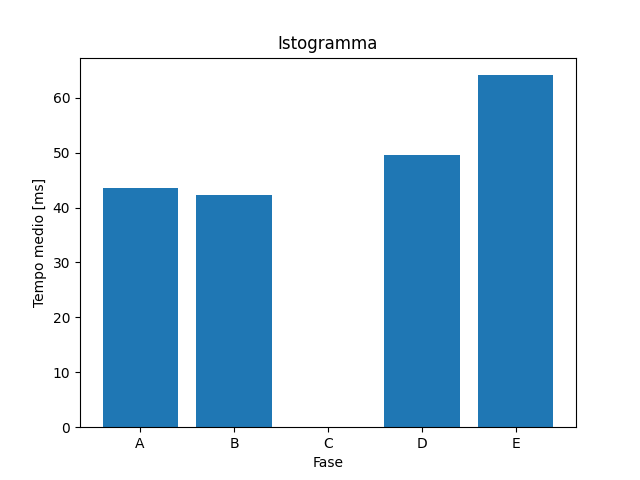
\includegraphics[width=\linewidth]{img/cap5/monolithic/istogramma.png}
		\end{subfigure}
		\caption{Boxplot e istogramma relativi ai tempi di esecuzione dell'applicazione monolitica}
		\label{fig:grafici-monolitica}
	\end{figure}
	
	\begin{figure}[tbp]
		\begin{subfigure}{0.5\textwidth}
			\centering
			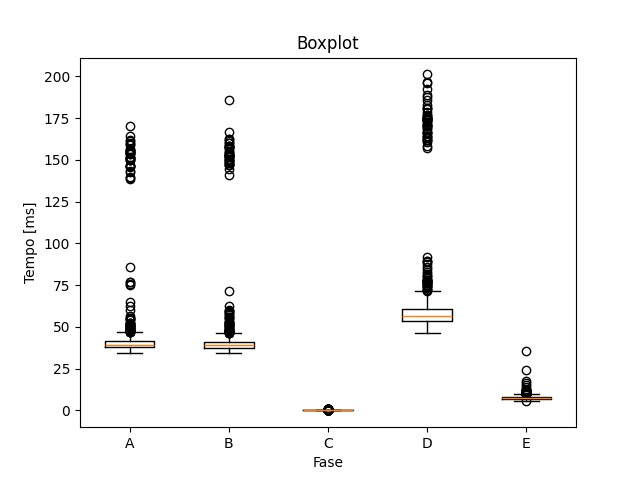
\includegraphics[width=\linewidth]{img/cap5/microservices/boxplot.png}
		\end{subfigure}
		\begin{subfigure}{0.5\textwidth}
			\centering
			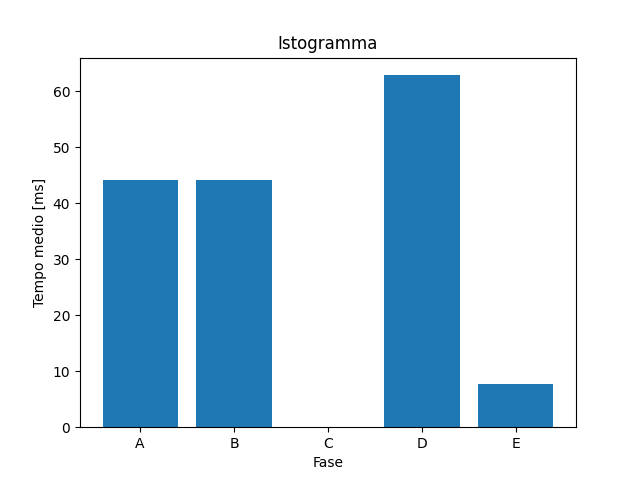
\includegraphics[width=\linewidth]{img/cap5/microservices/istogramma.png}
		\end{subfigure}
		\caption{Boxplot e istogramma relativi ai tempi di esecuzione dell'applicazione a microservizi}
		\label{fig:grafici-microserv}
	\end{figure}
	
	
	\chapter{Conclusioni e sviluppi futuri}

	In questo lavoro di tesi si è compiuto un confronto tra due due applicazioni realizzate seguendo approcci alla progettazione differenti, da un lato la modalità tradizionale di sviluppo, dall'altra una corrente emergente in crescita di anno in anno.
	
	L'utilizzo di Kubernetes rende più efficiente lo sviluppo e facilita la gestione del sistema, da sottolineare sono in particolari le caratteristiche di \emph{self-healing} e scalabilità offerte.
	
	Gli sviluppi futuri potrebbero essere molteplici e spaziare dall'ambito della sicurezza alla migrazione verso nuove tecnologie.
	L'aspetto sicurezza è indubbiamente di primaria importanza, le applicazioni sviluppate espongono infatti alla possibilità che un utente malevolo riesca ad impossessarsi di un token destinato a un altro utente, utilizzandolo per nascondere la propria identità.
	In secondo luogo la migrazione da PostgreSQL ad un database NoSQL porterebbe a un incremento della velocità di esecuzione delle query e permetterebbe la scalabilità orizzontale del sistema, aspetto di primaria importanza per un sistema distribuito.
	Valide alternative potrebbero essere MongoDB o Cassandra.
	Infine si potrebbe riscrivere l'intera applicazione in un linguaggio compilato: sebbene Python sia un linguaggio moderno, flessibile e sintetico, esso risulta essere uno dei linguaggi più lenti in esecuzione a causa della presenza dell'interprete;
	inoltre si presta bene solo per la scrittura di script o piccole applicazioni, altri linguaggi offrono un supporto molto maggiore alla programmazione in grande.
	L'utilizzo di un linguaggio compilato porterebbe in questo senso ad un buon incremento delle prestazioni.
	 
	
	\listoffigures
	\listoftables
	
	%% Bibliografia
	\printbibliography[heading=bibintoc]
%	\bibliography{biblio/biblio} 
%	\bibliographystyle{ieeetr}
	
\end{document}
